\documentclass[11pt]{article}

\usepackage[margin=1in]{geometry}
\usepackage{graphicx}
\usepackage{amsmath,amssymb}
\usepackage{booktabs}
\usepackage{microtype}
\usepackage{hyperref}
\usepackage{natbib}
\usepackage{authblk}

\title{Draphnet: Integrating Drug Bioassays and Disease Genetics to Map Drug
Impacts on the Human Phenome}

\author{}
\date{}

\begin{document}

\maketitle

\begin{abstract}
Unintended effects of approved medications remain a leading source of
both harm and opportunity: side effects burden patients and clinical
development, while unexpected therapeutic effects occasionally enable drug
repurposing. Connecting these effects to disease biology has been
difficult because predictive models for drug-disease relationships rarely
expose the molecular pathway from a drug's in vitro activity to the genes
that drive phenotype risk. We develop Draphnet, a supervised logistic
affinity-regression model that learns a single interaction network
linking drug bioassay endpoints to disease driver genes from three input
matrices: 429 compounds $\times$ 1391 ToxCast endpoints, 10,027 genes
$\times$ 197 UK Biobank phenotypes derived from PhenomeXcan/S-MultiXcan,
and a binary drug-phenotype annotation matrix from SIDER. We first show
that molecular and genetic similarity alone already capture strong
signal: drugs with similar ToxCast profiles share significantly more
phenotypes ($p=1\mathrm{e}{-22}$; linear model adjusted for shared
endpoints $p=1.7\mathrm{e}{-43}$), and diseases with more similar
PhenomeXcan profiles are perturbed by more similar sets of drugs
($p=4\mathrm{e}{-81}$). Draphnet's side-effect predictions on held-out
drugs outperform a nearest-neighbor baseline (rank-sum
$p=3\mathrm{e}{-8}$), and drugs sharing targets have significantly more
similar ToxCast endpoint effects ($p=1\mathrm{e}{-28}$). Most
importantly, projecting each drug through the learned network into a
10,027-gene disease-genome space recovers interpretable, target-level
enrichments: across 132 DrugBank targets shared by at least three drugs,
28 have disease genes associated at adjusted $p<0.01$, including PPM1M
for HTR2C-modulating neuroleptics and CETP for fenofibrate and other
PPAR$\alpha$-targeting drugs. Draphnet provides a biology-anchored view
of drug effects that is simultaneously predictive and mechanistically
interpretable.
\end{abstract}

\section{Introduction}

Thousands of drugs are approved and in widespread clinical use, and some
of their most important effects -- adverse reactions that only become
apparent post-marketing, or beneficial effects on diseases that were not
the original indication -- remain invisible to the predictive models that
accompanied their approval. Large observational resources such as SIDER
catalog post-approval side effects and indications at scale
\citep{kuhn2016sider}, and DrugBank and the Drug Repurposing Hub annotate
the molecular targets and therapeutic uses of thousands of compounds
\citep{knox2024drugbank,corsello2017repurposing}. On the molecular side,
high-throughput assays characterize how drugs perturb biology in
reproducible ways: the EPA ToxCast/Tox21 program assays hundreds of
compounds across more than a thousand biological endpoints
\citep{richard2016toxcast}, and the Connectivity Map and its L1000
successor profile drug-induced gene-expression signatures at large scale
\citep{lamb2006cmap,subramanian2017lincs}. Collectively, these resources
raise the prospect of reasoning systematically about which disease
processes a drug influences, and why.

In parallel, phenome-wide genetic studies have turned disease genetics
into a standardized, gene-level resource at unprecedented breadth. The UK
Biobank cohort provides genome-wide data for roughly half a million
participants and associated phenotypes \citep{bycroft2018ukbiobank}, and
gene-based methods such as PrediXcan, S-PrediXcan, and S-MultiXcan
integrate GWAS summary statistics with tissue-specific eQTL models to
move associations from variants to genes
\citep{gamazon2015predixcan,barbeira2018spredixcan,barbeira2019smultixcan},
with cross-tissue reference data supplied by the GTEx Consortium
\citep{gtex2020atlas}. PhenomeXcan consolidates these gene-level
associations for thousands of phenotypes into a queryable
gene-by-phenotype matrix \citep{pividori2020phenomexcan}.

Most prior computational approaches for uncovering unexpected drug
effects have exploited a single modality at a time. One family applies
the connectivity principle -- that effective drugs induce gene-expression
changes opposing the disease's molecular signature -- either directly
from cell-line expression data \citep{lamb2006cmap,sirota2011drugrepo}
or, more recently, from genetically imputed transcriptomes for selected
disorders \citep{so2017neuropsychiatric,reay2020pes,grotzinger2023tsem}.
A second family uses drug-side-effect similarity to infer shared targets
\citep{campillos2008sideeffect}. A third treats drug-disease prediction
as matrix completion on the incomplete drug-phenotype matrix. These
approaches have produced useful candidates, but they tend to be
predictive black boxes: they do not expose how the molecular effects of
a drug propagate through disease driver genes to produce phenotypic
effects, and therefore do not yield the mechanistic hypotheses that
clinicians and experimentalists most need.

Draphnet closes this gap by learning a single shared network that
connects drug molecular effects directly to disease driver genes. We
train a supervised logistic affinity-regression model that takes as
input the ToxCast drug-endpoint matrix $D$, the PhenomeXcan
gene-by-phenotype matrix $P$, and the SIDER drug-by-phenotype binary
matrix $Y$, and learns an interaction matrix $W$ such that $DWP^{\top}$
approximates $\mathrm{logit}(p(Y))$. The same $W$ is shared across
thousands of drug-phenotype pairs, enforcing the prior that the
biological wiring from endpoints to disease genes is largely common
across contexts. By imposing sparsity through $L_1$ regularization and
handling the high dimensionality and missingness of $D$ and $P$ through
SoftImpute \citep{mazumder2010softimpute} and singular-value
decomposition respectively, we adapt the affinity-regression framework
originally developed for signaling-to-transcription networks
\citep{osmanbeyoglu2014affinity} to a binary, multitask drug-phenotype
setting. Phenotype names are harmonized between UK Biobank and SIDER
through UMLS concept unique identifiers \citep{bodenreider2004umls}.

We make three contributions. First, we establish the premise that
molecular and genetic similarity alone already carry strong signal for
drug-disease biology, quantified across all pairs of drugs and all
pairs of phenotypes in our data. Second, we show that Draphnet's
learned model generalizes to held-out drugs and significantly
outperforms a nearest-neighbor baseline in the same feature space.
Third, by projecting each drug through the learned network into a
10,027-gene disease-genome space, we recover mechanistically
interpretable target-level enrichments and surface specific drug-gene
associations -- including PPM1M for HTR2C-modulating neuroleptics and
CETP for fenofibrate and other PPAR$\alpha$-targeting drugs -- that are
consistent with prior experimental evidence on PPAR$\alpha$-family
regulation \citep{huang2022perm1}. We present Draphnet as both a
predictive model for drug-phenotype relationships and a resource for
generating testable biological hypotheses for drug repurposing.

\section{Related work}

Connectivity-based drug repurposing has repeatedly shown that shared
gene-expression responses can link drugs and diseases. The original
Connectivity Map \citep{lamb2006cmap} and its L1000 successor
\citep{subramanian2017lincs} motivated a large downstream literature,
including cross-modality extensions such as discovery of new indications
from public gene-expression compendia \citep{sirota2011drugrepo}. More
recent work has extended the idea to genetically imputed transcriptomes
via S-PrediXcan-style models, yielding neuropsychiatric repurposing
candidates \citep{so2017neuropsychiatric,reay2020pes} and, most
recently, cross-disorder repurposing via transcriptome-wide structural
equation modeling across 13 psychiatric disorders
\citep{grotzinger2023tsem}. These methods, while informative, are
either tied to narrow disease families or operate on gene-expression
signatures rather than on GWAS-derived disease-driver genetics, and
they do not learn an interpretable drug-to-gene network.

A complementary line uses drug-phenotype similarity to infer drug-target
relationships. The finding that side-effect similarity is predictive of
shared molecular targets \citep{campillos2008sideeffect} has been
extended with matrix-completion and graph-based approaches for
drug-target interaction prediction. These methods predict missing
drug-disease annotations or targets, but they do not expose the
underlying drug-endpoint-to-disease-gene wiring.

Finally, methodological work on polypharmacology has emphasized that
most effective drugs act on multiple proteins and that meaningful
drug-biology models must allow for this complexity
\citep{hopkins2008network}. This observation is directly relevant to how
we interpret Draphnet: targets such as CHRM1, annotated as a target of
14 mechanistically diverse compounds, are unlikely to produce a
homogeneous phenome-effect signature, and our target-level tests are
designed to tolerate this heterogeneity. Statistical control across
thousands of correlated gene-level tests per drug is handled by
Benjamini-Yekutieli-adjusted empirical permutation
\citep{benjamini2001fdrdependency,benjamini1995fdr}, and graph
analyses for the drug-drug overlap network are performed with NetworkX
\citep{hagberg2008networkx}.

\section{Materials and Methods}

\subsection{Data and matrices}

We assemble three matrices that are shared across all experiments in
this paper (Figure~\ref{fig:schematic} illustrates how they combine).
The drug-endpoint matrix $D$
is compiled from ToxCast Level~5 data \citep{richard2016toxcast} and
contains 429 compounds scored over 1391 endpoints, where each entry is
the fraction of models that called the compound a hit. $D$ is sparse:
on average, each drug is assayed for approximately 100 endpoints, and
the remaining entries are missing. The gene-phenotype matrix $P$ is
compiled from PhenomeXcan \citep{pividori2020phenomexcan}, which
integrates UK Biobank GWAS summary statistics with tissue-specific eQTL
models via S-PrediXcan and S-MultiXcan
\citep{barbeira2018spredixcan,barbeira2019smultixcan}. We convert each
S-MultiXcan $p$-value to a signed $z$-score using
$|\Phi^{-1}(p_{\text{multiXcan}})| \times \mathrm{sign}$, where the
sign is the consensus S-PrediXcan sign across tissues, yielding a
phenotype-association score for each gene. We retain the top half of
genes by across-phenotype standard deviation, giving $P$ with 10,027
genes and 197 phenotypes. The binary drug-phenotype matrix $Y$ is
compiled from SIDER \citep{kuhn2016sider} and encodes, for each drug,
the phenotypes listed as either indications or side effects; phenotype
names are harmonized between UK Biobank and SIDER using UMLS concept
unique identifiers \citep{bodenreider2004umls}. Table~\ref{tab:matrices}
summarizes dimensions and sources.

\begin{table}[htbp]
\centering
\caption{Summary of input matrices for Draphnet.}
\label{tab:matrices}
\begin{tabular}{llll}
\toprule
Matrix & Meaning & Dimensions & Source \\
\midrule
$D$ & Drug $\times$ endpoint (fraction hit, with missing entries) & $429 \times 1391$ & ToxCast/Tox21 Level~5 \\
$P$ & Gene $\times$ phenotype (signed $z$-score) & $10{,}027 \times 197$ & PhenomeXcan / S-MultiXcan \\
$Y$ & Drug $\times$ phenotype (binary) & $429 \times 197$ & SIDER (matched via UMLS) \\
$U_D S_D$ & Low-rank SoftImpute projection of $D$ & $429 \times r_D$ & SoftImpute on $D$ \\
$W_{DP}$ & Learned interaction matrix (factored space) & $r_D \times r_P$ & Logistic affinity regression \\
\bottomrule
\end{tabular}
\end{table}

% Figure 1: schematic embedded near its first mention
\begin{figure}[htbp]
\centering

\includegraphics[width=0.85\textwidth]{figures/fig_schematic.pdf}
\caption{Draphnet integrates three input matrices into a single logistic
affinity-regression model. The drug-by-endpoint matrix $D$ (429 compounds
$\times$ 1391 ToxCast endpoints) is dimensionality-reduced via SoftImpute
to $U_D S_D$; the gene-by-phenotype matrix $P$ (10{,}027 genes $\times$ 197
UK Biobank phenotypes from PhenomeXcan) is reduced via singular-value
decomposition; and a shared interaction matrix $W_{DP}$ is trained by
$L_1$-regularized logistic regression to predict the binary drug-phenotype
annotation matrix $Y$ from SIDER.}
\label{fig:schematic}
\end{figure}

\subsection{Model and dimensionality reduction}

We adapt affinity regression \citep{osmanbeyoglu2014affinity} to a
binary outcome. In its bilinear form, the model posits that
\begin{equation}
D W P^{\top} = \mathrm{logit}(p(Y)),
\label{eq:bilinear}
\end{equation}
so that $W$ is a single interaction matrix that propagates drug-endpoint
effects through disease-driver-gene effects to produce phenotypic
probabilities. Because $D$ has missing entries and many correlated
endpoints, we first project it to a lower-dimensional
representation $U_D S_D$ using SoftImpute
\citep{mazumder2010softimpute}. SoftImpute's rank and regularization are
selected by a cross-validation-like procedure that masks 5\% of
non-missing entries and minimizes the imputation mean squared error on
the masked cells. Pairwise similarity is well preserved after
dimensionality reduction: the Spearman correlation between drug-pair
similarity in $D$-space and in $U_D S_D$-space is $0.21$. We further
decompose $P$ by singular-value decomposition as
$P = U_P S_P V_P^{\top}$. Substituting both decompositions into
Equation~\ref{eq:bilinear} and applying the Kronecker identity yields
the standard regression
\begin{equation}
(V_P \otimes (U_D S_D))\, \mathrm{stack}(W_{DP}) = \mathrm{logit}(p(Y)),
\label{eq:kron}
\end{equation}
which we solve with $L_1$-regularized logistic regression. The
regularization parameter is tuned by holding out 10\% of drugs per
cross-validation fold. Our final selected hyperparameters are
$r_P = 131$, $r_D = 95$, and lasso regularization $= 1$. Table~\ref{tab:hparams}
summarizes the full set of cross-validation and null-distribution
settings used in this paper.

\begin{table}[htbp]
\centering
\caption{Hyperparameters, cross-validation settings, and multiple-testing
controls for Draphnet. All hyperparameters are selected by held-out-drug
cross-validation.}
\label{tab:hparams}
\begin{tabular}{ll}
\toprule
Setting & Value \\
\midrule
SVD rank of $P$ ($r_P$) & $131$ \\
SoftImpute rank of $D$ ($r_D$) & $95$ \\
Lasso logistic regularization & $1$ \\
Drug fraction held out per CV fold (prediction evaluation) & $5\%$ \\
Drug fraction held out per CV fold (regularization tuning) & $10\%$ \\
Number of CV folds (prediction comparison) & $20$ \\
Entries masked for SoftImpute hyperparameter tuning & $5\%$ of non-missing \\
Permutations of $Y$ for drug-disease-genome null & $10{,}000$ \\
Clique-null simulations (disease-gene overlap) & $1{,}000$ \\
Multiple-testing correction (drug-gene $p$-values) & Benjamini-Yekutieli \\
Multiple-testing correction (target enrichment) & Benjamini-Hochberg \\
\bottomrule
\end{tabular}
\end{table}

\subsection{Prediction evaluation}

We evaluate predictive performance by 20-fold cross-validation over
drugs, where within each fold 5\% of drugs are held out and their SIDER
side-effect profiles are predicted from Draphnet trained on the
remaining data. As a baseline, we predict each held-out drug's profile
by its nearest neighbor in $D$-space. The two methods are compared by
Jaccard distance between predicted and actual profiles, and the
hypothesis that Draphnet achieves lower Jaccard distance than the
nearest-neighbor baseline is tested by rank-sum test.

\subsection{Phenome-effect and disease-genome projections}

After fitting Draphnet, we compute the drug phenome-effect matrix
$U_D S_D W_{DP}$, which maps each drug to a compressed summary of its
effects across the phenome. We further project this quantity into the
full $10{,}027$-gene disease-genome space by applying the inverses of
the SVD of $P$, which yields a drug-by-gene matrix whose entries
represent, for each drug, its estimated impact on each disease driver
gene.

\subsection{Empirical permutation null and multiple testing}

To decide which drug-gene entries reflect the learned interaction
matrix rather than structure that is already present in the input data,
we construct an empirical null by permuting the entries of $Y$,
refitting the full pipeline, and recomputing the drug-gene matrix. We
perform 10,000 such permutations and assign empirical $p$-values to
every drug-gene cell. Because the $\sim$10,027 tests per drug are
correlated, $p$-values are adjusted using the Benjamini-Yekutieli
procedure \citep{benjamini2001fdrdependency}. For target-level
enrichment tests, we ask, for each DrugBank target, whether drugs
sharing that target are enriched for particular significant disease
genes; $p$-values from the hypergeometric test are adjusted with the
Benjamini-Hochberg procedure \citep{benjamini1995fdr}. A second
permutation null, in which drug-target labels are scrambled, is used to
calibrate the overall significance of target-level enrichments
(Figure~3A of the Results text).

\subsection{Drug-drug cliques}

To produce a novel drug categorization based on shared effects on the
disease genome, we construct a weighted random null by sampling, for
each drug, a set of disease genes with probability proportional to the
number of drugs each gene is significantly associated with. Repeating
this simulation 1,000 times yields a nominal significance threshold for
the overlap of disease genes between any pair of drugs. We connect
pairs of drugs whose true overlap exceeds this threshold, then identify
all fully connected cliques of at least three drugs using NetworkX
\citep{hagberg2008networkx}; bipartite visualization of drugs and
disease genes uses igraph.

\section{Results}

\subsection{Drug molecular similarity and disease genetic similarity both
track phenotypic overlap}

We begin by establishing the premise that drug-disease biology is
reflected in the inputs to Draphnet before any supervised training. For
each pair of the 429 drugs, we compute the Jaccard similarity of their
SIDER profiles and the Spearman correlation of their ToxCast endpoint
scores over endpoints where both drugs were assayed. If ToxCast
profiles carry any signal about phenotypes, pairs of drugs with more
correlated endpoint profiles should share more SIDER phenotypes.

Across all drug pairs, this relationship is strongly significant: the
Spearman correlation between Jaccard similarity of phenotypes and
Spearman correlation of endpoint profiles is associated at
$p=1\mathrm{e}{-22}$, and a linear model that additionally adjusts for
the number of shared endpoints (to rule out trivial effects of assay
coverage) strengthens this signal to $p=1.7\mathrm{e}{-43}$. The
relationship therefore persists after accounting for how much ToxCast
overlap two drugs happen to have, suggesting that endpoint profiles
themselves carry the relevant information. Dimensionality reduction
does not destroy this structure: the Spearman correlation between drug
pairwise similarity computed from the raw $D$ and from the
SoftImpute-projected $U_D S_D$ is $0.21$, indicating that the
low-rank representation we will feed into Draphnet preserves the
similarity geometry of the input.

The analogous test on the phenotype side yields the same qualitative
picture. For each pair of phenotypes, we compute the Jaccard index of
their associated drug sets in SIDER and the Spearman correlation of
their PhenomeXcan gene-association profiles. Phenotypes with more
similar PhenomeXcan profiles are perturbed by more similar drug sets at
$p=4\mathrm{e}{-81}$, with an aggregate disease-pair Spearman
correlation of $-0.11$ between Jaccard distance and PhenomeXcan profile
correlation. Taken together, these two tests motivate the premise of
the model: drugs and diseases that are close in their respective
molecular or genetic spaces are also close in drug-disease space, and a
learned network connecting these spaces should therefore be able to
exploit both sides of the similarity structure simultaneously.

\subsection{Draphnet predictions generalize to held-out drugs and
outperform a nearest-neighbor baseline}

We next ask whether the full Draphnet model learns anything beyond the
similarity structure already present in its inputs. With
cross-validated hyperparameters $r_P = 131$, $r_D = 95$, and lasso
regularization $=1$, we train Draphnet in a 20-fold cross-validation
over drugs (5\% held out per fold) and compare its predicted side-effect
profiles to those produced by the simplest comparable baseline, a
nearest-neighbor classifier that predicts each held-out drug's
side-effect profile from its nearest neighbor in $D$-space.

For a majority of held-out drugs, Draphnet achieves lower Jaccard
distance between predicted and observed side-effect profiles than the
nearest-neighbor baseline. The difference is strongly significant by
rank-sum test ($p=3\mathrm{e}{-8}$, Figure~\ref{fig:prediction}). This
comparison is conservative: both Draphnet and the baseline receive the
same input features, so any improvement must come from the learned
interaction network rather than from better inputs.

\begin{figure}[htbp]
\centering
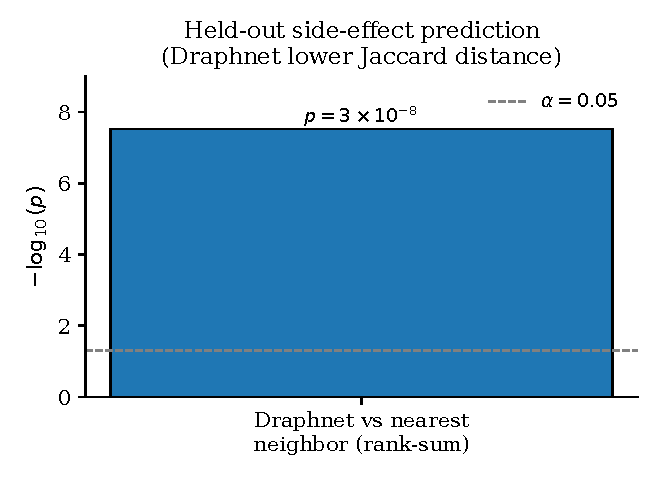
\includegraphics[width=0.55\textwidth]{figures/fig_prediction.pdf}
\caption{Held-out side-effect prediction. On a 20-fold cross-validation
over drugs (5\% held out per fold), Draphnet produces lower Jaccard
distance between predicted and observed SIDER profiles than a
nearest-neighbor baseline trained in the same $D$ space (rank-sum
$p=3\times 10^{-8}$). Dashed line marks the $\alpha=0.05$ significance
threshold.}
\label{fig:prediction}
\end{figure}

Several off-label top predictions are biologically plausible.
Fludrocortisone is ranked as the top non-indicated predicted treatment
for eczema; the drug is an oral corticosteroid, whereas eczema is
typically treated by topical steroids, so the prediction aligns with
known biology despite a different administration route. Methyclothiazide,
a diuretic, is the top non-indicated predicted treatment for glaucoma;
because glaucoma's primary cause is fluid retention in the eye, this is
a mechanistically plausible off-label prediction. Finally, dasatinib's
top predicted indications are cancers, even though its primary indication
(leukemia) is absent from the training matrix $P$ and could not be
learned directly. Together, these examples indicate that the held-out
predictions are not only statistically better than baseline but are
also clinically interpretable.

\subsection{The drug phenome-effect matrix recapitulates known drug
biology}

Prediction, however, is not the central aim of Draphnet; the more
important test is whether the learned interaction matrix captures
biology beyond what is already present in $D$. To ask this, we project
each drug through $U_D S_D W_{DP}$ to obtain its phenome-effect vector
and compare pairs of drugs that share known molecular targets to those
that do not. We first verify the sanity check that drugs sharing one or
more DrugBank targets have more similar raw ToxCast endpoint effects
than drugs that do not (rank-sum $p=1\mathrm{e}{-28}$): if this were
not the case, no downstream projection could recover target structure.

The critical test is then whether the true phenome-effect projection
distinguishes drugs that share targets more effectively than a null
projection in which the interaction matrix is replaced by a permuted
version. For most targets, it does: on a per-target $-\log_{10}(p)$
scale, the majority of DrugBank targets sit above the identity line
(true enrichment $>$ null enrichment), confirming that the learned $W$
adds target-relevant structure that is not already present in the
ToxCast inputs. Among drug pairs that share a target, the Spearman
correlation of their phenome-effect vectors is systematically higher in
the true projection than in the null projection; the effect is
significant for many individual target classes, with several crossing
the $p<10^{-5}$ threshold. We emphasize that both comparisons hold the
input data fixed and vary only the interaction matrix, so any
improvement can be attributed specifically to the model and not to
structure that was already present in $D$.

A small number of target classes do not show improvement, and these
exceptions are themselves biologically informative. CHRM1, for
instance, is annotated as a target of 14 drugs spanning
anticholinergics, neuroleptics, migraine treatments, and ophthalmological
preparations; these 14 drugs carry a median of 19 other targets. The
resulting phenome-effect vectors cannot be expected to cluster
tightly, because CHRM1 activity is embedded in very different
polypharmacological contexts -- precisely the situation that motivated
the move from single-target models toward network pharmacology
\citep{hopkins2008network}. Having verified that the learned
interaction matrix captures target-relevant biology on average while
failing gracefully on heavily polypharmacological targets, we now ask
the question the method was built to answer: which specific disease
driver genes does each drug impact?

\subsection{Projecting drugs onto the disease genome reveals target-level
enrichments of disease driver genes}

Having validated that the learned interaction matrix encodes
target-relevant signal, we proceed to the primary interpretive output
of Draphnet: projecting each drug into the full 10,027-gene
disease-genome space and identifying, per drug, the disease genes that
its molecular profile is expected to impact. Significance for each
drug-gene entry is assessed against an empirical null built from 10,000
permutations of $Y$ followed by full model refitting, and adjusted per
drug using the Benjamini-Yekutieli procedure to account for correlation
among the $\sim$10,027 gene-level tests.

After adjustment, we obtain a median of seven disease genes per drug.
At the target level, across 132 DrugBank targets shared by at least
three drugs in our set, 28 targets have one or more significantly
associated disease genes at adjusted $p<0.01$
(Figure~\ref{fig:enrichment}).

\begin{figure}[htbp]
\centering
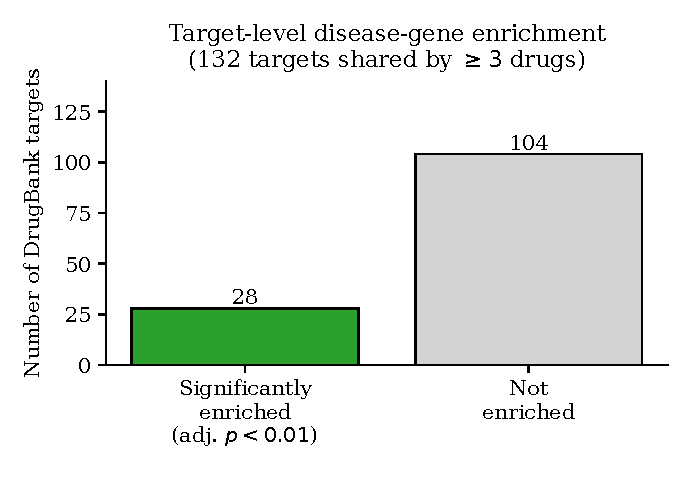
\includegraphics[width=0.55\textwidth]{figures/fig_enrichment.pdf}
\caption{Target-level enrichment of disease-gene associations. Of 132
DrugBank targets that are shared by at least three drugs in our set, 28
($\approx$21\%) have one or more disease genes significantly associated
with drug-target membership at Benjamini-Hochberg-adjusted $p<0.01$.}
\label{fig:enrichment}
\end{figure}

A target-level calibration plot
comparing true drug-target enrichments to those obtained under
permuted drug-target labels shows that the true significance values are
systematically larger than the null (Fig.~3A of the Results figure
legends): drug-target enrichments are therefore unlikely to be explained
by chance, and they are not artifacts of $D$ alone because the null
uses the same input data but scrambles the learned relation between
drug and target.

The resulting drug-disease-gene assignments carry concrete biological
content (Figure~\ref{fig:associations}).

\begin{figure}[htbp]
\centering
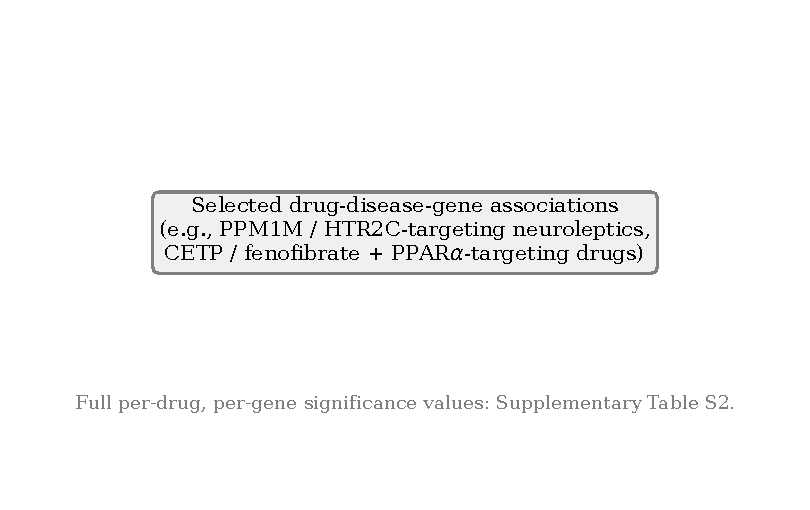
\includegraphics[width=0.7\textwidth]{figures/fig_associations.pdf}
\caption{Representative drug-disease-gene associations identified by
Draphnet, including PPM1M for HTR2C-targeting neuroleptics and CETP for
fenofibrate and other PPAR$\alpha$-targeting drugs. Per-drug significance
values are provided in Supplementary Table~S2; this figure summarizes
the categories discussed in the main text.}
\label{fig:associations}
\end{figure}

A $t$-SNE visualization of
drug target-significance profiles shows that drugs in the same ATC
therapeutic subgroup cluster together: calcium channel blockers form
one cluster, and anti-inflammatories/analgesics form another (Fig.~3B
of the Results figure legends). Two specific drug-gene links highlight
the hypothesis-generating potential of the approach. First, PPM1M is
associated with several HTR2C-targeting neuroleptics (drugs that
modulate serotonin signaling); it is the top PhenomeXcan gene for
bipolar disorder, a recent schizophrenia GWAS reported a locus in this
gene, and an independent study linked the locus to rare mental illness,
so the Draphnet association converges with external genetic evidence.
Second, CETP (cholesterol ester transfer protein) is associated with
fenofibrate and other drugs targeting lipid metabolism. CETP is
associated with high cholesterol in PhenomeXcan, and prior experimental
work supports CETP as an effector of fenofibrate and
PPAR$\alpha$ agonism \citep{huang2022perm1}. In both cases, Draphnet
recovers a drug-gene link that would be difficult to pick out from
either the drug-endpoint data or the disease-gene data in isolation.

\subsection{A novel drug categorization based on shared disease-gene
effects}

The drug-disease-genome matrix also supports categorizations of drugs
that cut across pharmacology and clinical indication. We build a
drug-drug graph by connecting pairs of drugs whose overlap in
significant disease genes exceeds a weighted random null (1,000
simulations, sampling disease genes in proportion to the number of
drugs each is associated with). We then identify fully connected
cliques of at least three drugs with NetworkX and visualize the
resulting bipartite drug-gene graph with igraph (Fig.~4 of the
Results figure legends), retaining only disease genes associated with
at least one gene target and with fewer than 15 total drugs.

Some cliques recover expected groupings. Ketoprofen, ibuprofen, and
indomethacin -- three canonical anti-inflammatories -- cluster together,
and their clique extends to PPAR$\alpha$-agonists (fenofibrate and
bezafibrate), consistent with the known anti-inflammatory activity of
PPAR$\alpha$-agonists. Pyridoxine (vitamin B-6) appears in the same
clique, consistent with its own anti-inflammatory effects. Other
cliques are unexpected but mechanistically plausible. A clique of
calcium channel blockers (bepridil, verapamil) connects to pimozide, a
psychiatric drug known to cause arrhythmia as a side effect; this
connection is particularly interesting because pimozide's adverse
cardiac profile overlaps mechanistically with the primary action of
calcium channel blockers. A further clique links mecamylamine -- a
largely discontinued antihypertensive whose discontinuation was driven
in part by central nervous system effects -- to pindolol (an
antihypertensive beta blocker) and gabapentin (a central nervous
system drug for seizures and nerve pain); mecamylamine has more
recently been investigated for seizure and behavioral disorders,
consistent with its position in this clique. We present these
categorizations as hypothesis-generating resources rather than as
validated groupings.

\section{Discussion}

Our results show that it is possible to train a single, interpretable
network that simultaneously predicts drug-phenotype associations and
exposes the disease-gene machinery by which drug molecular effects
could produce those associations. Draphnet operates on three
large-scale resources -- ToxCast bioassays, PhenomeXcan gene-based
phenome data, and SIDER drug-phenotype annotations -- that were
previously used in isolation, and it learns a shared interaction
matrix that is portable across thousands of drug-phenotype pairs. The
model's predictions on held-out drugs significantly outperform a
nearest-neighbor baseline trained in the same feature space, and,
more importantly, the projection of each drug into a 10,027-gene
disease-genome space recovers target-level enrichments that are
concordant with known pharmacology (for instance, calcium channel
blockers cluster together in ATC-aware $t$-SNE; anti-inflammatories
link to PPAR$\alpha$-agonists) while also surfacing novel candidate
mechanisms.

Several aspects of the results align with, and extend, prior
computational drug-repurposing work. Connectivity-based methods
\citep{lamb2006cmap,subramanian2017lincs,sirota2011drugrepo} and their
GWAS-informed extensions
\citep{so2017neuropsychiatric,reay2020pes,grotzinger2023tsem} have
established that gene-expression or genetic proxies for disease biology
can be used to prioritize drugs, but they generally stop at
drug-disease scores. Draphnet adds a mechanistic layer: for each
drug-disease pair, we can decompose the predicted relationship into
the disease driver genes through which it flows. This is the same
modeling philosophy that underlies affinity regression in
transcriptional biology \citep{osmanbeyoglu2014affinity}, adapted here
from continuous expression outputs to binary drug-phenotype outcomes
through logistic regression.

The specific drug-gene links we recover are consistent with independent
biological evidence and illustrate how the model can generate testable
hypotheses. CETP's association with fenofibrate and related
PPAR$\alpha$-targeting drugs is consistent with experimental work
demonstrating that PERM1 and related factors co-regulate
PPAR$\alpha$-responsive genes in a way that can plausibly affect
cholesterol metabolism \citep{huang2022perm1}. PPM1M's association
with HTR2C-modulating neuroleptics is consistent with recent
psychiatric GWAS that implicate the same locus in schizophrenia and
rare mental illness, and it agrees qualitatively with the
observation that drug-side-effect similarity is predictive of shared
molecular targets \citep{campillos2008sideeffect}. Drug cliques
that cross therapeutic categories -- such as anti-inflammatories
linked to PPAR$\alpha$-agonists, or mecamylamine linked to gabapentin
and pindolol -- show that the method can recover the kind of
polypharmacologically motivated groupings that network pharmacology
has argued should exist \citep{hopkins2008network}.

Several limitations must be acknowledged. First, the training matrix
$Y$ is intrinsically incomplete: SIDER captures only the drug-phenotype
associations that have been documented, so our putative negatives
include an unknown number of latent true positives. Accuracy is
therefore not the ideal metric for evaluating the model, and the
magnitude of the Draphnet--nearest-neighbor gap we report should be
read as a conservative lower bound. Second, the mapping from GWAS loci
to disease genes is itself uncertain; for example, the long non-coding
RNA RP11-54O7.17 appears as a disease gene linked to
PPAR$\gamma$-agonists, while the adjacent gene PERM1, an experimentally
supported PPAR$\gamma$ effector \citep{huang2022perm1}, has fewer
recorded eQTLs in the tissues covered by GTEx \citep{gtex2020atlas} and
therefore less signal in PhenomeXcan. Comprehensive resources that
supplement eQTL-based mapping with other gene-disease evidence can be
expected to improve the disease-gene layer of Draphnet. Third, despite
our use of cross-validation, regularization, and aggressive
dimensionality reduction, the training data are small relative to the
number of parameters the model could in principle estimate; results
should therefore be considered exploratory at the level of individual
drug-gene associations, though the aggregate target-level enrichments
are statistically strong.

Several extensions follow naturally. The LINCS Connectivity Map
\citep{subramanian2017lincs} provides a systematic drug-by-cell-line
perturbation resource that could augment or replace the ToxCast side
of $D$ with gene-expression signatures, enabling a direct comparison
between bioassay-based and transcriptomic drug representations within
the same Draphnet framework. Projecting the drug phenome-effect
matrix onto biological pathways rather than individual genes would
allow pathway-level drug comparisons and could clarify how apparently
unrelated diseases come to share drug-mediated mechanisms. On the
statistical side, our empirical nulls are computationally intensive
but unbiased; more efficient analytical nulls would enable much larger
experiments, including extensions to individual-level risk allele
profiles that would connect Draphnet directly to personalized
medicine.

More broadly, Draphnet illustrates that two of the most powerful
resources in modern pharmacogenomics -- systematic drug bioassays and
phenome-wide gene-level GWAS -- can be linked by a supervised,
interpretable model that operates at the scale of the full drug-disease
space. The learned interaction matrix is a compact, reusable object
that can be queried for any new drug or disease and that provides a
principled place to insert biological prior knowledge (for example,
pathway- or tissue-specific structure) in future work. We expect the
approach to accelerate the generation of mechanistic hypotheses for
drug side effects and repurposing, and to lay a foundation for
individualized analyses in which a single patient's risk allele
profile can be projected through the same network. In the longer
term, because the disease genome half of Draphnet is pegged to
phenome-wide GWAS rather than to a fixed disease taxonomy, the model
will inherit the gains of ongoing biobank growth and eQTL refinement,
and the drug half can be swapped for or augmented with richer
perturbation data from LINCS, CRISPR screens, or multi-tissue
pharmacogenomic panels -- turning Draphnet into a living map from
compound libraries to human phenotype risk.

\bibliographystyle{plainnat}
\bibliography{references}

\end{document}
